\documentclass[a4paper]{article}

\usepackage[margin=1in]{geometry} % full-width

\usepackage{amsmath}
\usepackage{amsthm}
\usepackage{amssymb}

\usepackage[backend=biber, style=numeric]{biblatex}
\addbibresource{refs.bib}


\usepackage{graphicx, color}
\graphicspath{{fig/}}
\usepackage{algorithm, algpseudocode}
\usepackage{mathrsfs}
\usepackage{hyperref}

\usepackage{pgfplots}
\pgfplotsset{compat=1.14}
\usepgfplotslibrary{fillbetween}
\usetikzlibrary{intersections}


\title{Comparación de Técnicas de Integración Numérica}
\author{Nicolás Gómez Aragón\thanks{\texttt{nicolas.gomeza@javeriana.edu.co}}}
\date{Pontificia Universidad Javeriana\\\vspace{0.5cm}\today}


\begin{document}
	\maketitle
	
	\begin{abstract}
		El propósito de este proyecto es llevar a cabo una evaluación y comparación de técnicas de integración numérica empleando funciones de prueba como referencia. Se investigarán métodos como la regla del trapecio, la regla de Simpson y la cuadratura gaussiana. Estas técnicas se implementarán en Python, y se llevará a cabo un análisis de sus resultados en términos de precisión y eficiencia computacional.
	
		\noindent\textbf{Palabras Clave:} Integración, Eficiencia, computacional.
	\end{abstract}

	\tableofcontents
	
	\section{Resumen del Proyecto}
	\label{sec:resumen}
	
	El objetivo de este proyecto es evaluar y comparar la precisión y eficiencia de varias técnicas de integración numérica utilizando funciones de prueba. Se explorarán métodos como la regla del trapecio, la regla de Simpson y la cuadratura gaussiana. Estas técnicas se implementarán en Python y se analizarán sus resultados en términos de precisión y eficiencia computacional.
	
	\section{Objetivos del Proyecto}
	\label{sec:objetivos}
	\begin{itemize}
		\item Profundizar en temas introductorios de análisis numérico y técnicas de integración numérica.
		\item Familiarizarse con implementaciones de métodos numéricos en Python para problemas de cálculo.
		\item Comprender conceptos clave como precisión y eficiencia computacional.
	\end{itemize}


	\section{Técnicas de Integración Numérica}
	\label{sec:tecnicas}
    A continuación se describen las tres técnicas de integración las cuales serán estudiadas en  este artículo.

    \subsection{Regla del Trapecio}
    La \textbf{Regla del Trapecio} es un método de aproximación numérica para calcular el valor de una integral definida. Se basa en dividir el área bajo una curva en múltiples trapecios y sumar sus áreas para estimar la integral. Para una función $f(x)$ en el intervalo $[a, b]$, la fórmula de la Regla del Trapecio se expresa de la siguiente manera:

    \[
    \int_{a}^{b} f(x) dx \approx \frac{b-a}{2} \left[f(a) + f(b)\right]
    \]
    
    donde $\frac{b-a}{2}$ es el ancho del trapecio y $\left[f(a) + f(b)\right]$ representa la suma de las alturas de los 
    extremos. Este método es simple, lo cual lo hace no muy preciso para funciones complicadas.
    
    
    \begin{center}
    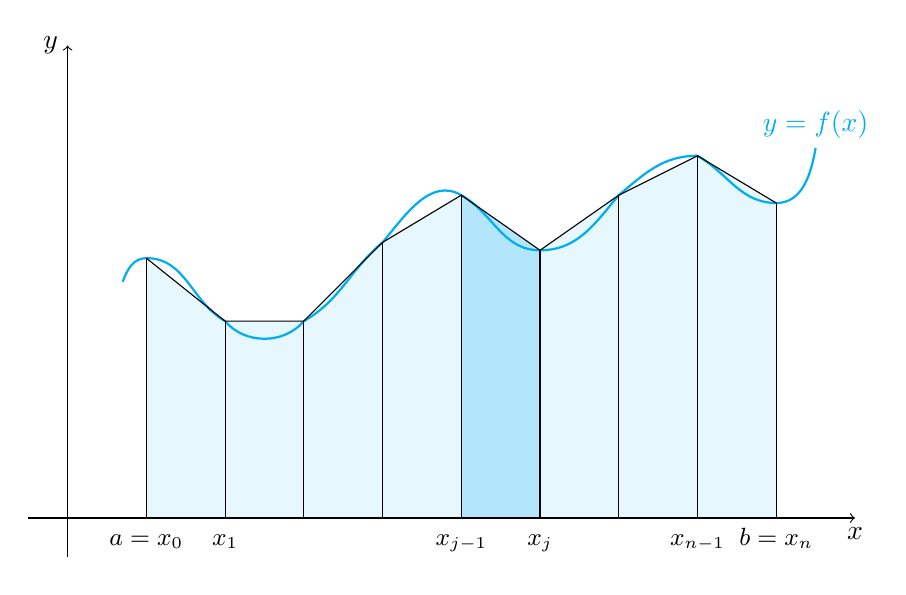
\begin{tikzpicture}
        \coordinate (p1) at (0.7,3);
        \coordinate (p2) at (1,3.3);
        \coordinate (p3) at (2,2.5);
        \coordinate (p4) at (3,2.5);
        \coordinate (p5) at (4,3.5);
        \coordinate (p6) at (5,4.1);
        \coordinate (p7) at (6,3.4);
        \coordinate (p8) at (7,4.1);
        \coordinate (p9) at (8,4.6);
        \coordinate (p10) at (9,4);
        \coordinate (p11) at (9.5,4.7);
        
        % The cyan background
        \fill[cyan!10] 
          (p2|-0,0) -- (p2) -- (p3) -- (p4) -- (p5) -- (p6) -- (p7) -- (p8) -- (p9) -- (p10) -- (p10|-0,0) -- cycle;
        % the dark cyan stripe
        \fill[cyan!30] (p6|-0,0) -- (p6) -- (p7) -- (p7|-0,0) -- cycle;
        % the curve
        \draw[thick,cyan] 
          (p1) to[out=70,in=180] (p2) to[out=0,in=150] 
          (p3) to[out=-50,in=230] (p4) to[out=30,in=220] 
          (p5) to[out=50,in=150] (p6) to[out=-30,in=180] 
          (p7) to[out=0,in=230] (p8) to[out=40,in=180] 
          (p9) to[out=-30,in=180] (p10) to[out=0,in=260] (p11);
        % the broken line connecting points on the curve
        \draw (p2) -- (p3) -- (p4) -- (p5) -- (p6) -- (p7) -- (p8) -- (p9) -- (p10);
        % vertical lines and labels
        \foreach \n/\texto in {2/{a=x_0},3/{x_1},4/{},5/{},6/{x_{j-1}},7/{x_j},8/{},9/{x_{n-1}},10/{b=x_n}}
        {
          \draw (p\n|-0,0) -- (p\n);
          \node[below,text height=1.5ex,text depth=1ex,font=\small] at (p\n|-0,0) {$\texto$};
        }
        % The axes
        \draw[->] (-0.5,0) -- (10,0) coordinate (x axis);
        \draw[->] (0,-0.5) -- (0,6) coordinate (y axis);
        % labels for the axes
        \node[below] at (x axis) {$x$};
        \node[left] at (y axis) {$y$};
        % label for the function
        \node[above,text=cyan] at (p11) {$y=f(x)$};
    \end{tikzpicture}
    \end{center}

    \subsection{Regla de Simpson}
    La \textbf{Regla de Simpson} es un método más preciso que la Regla del Trapecio para la 
    aproximación numérica de una integral definida. Utiliza polinomios de segundo grado para 
    ajustar la curva de la función. La fórmula de la Regla de Simpson se expresa de la siguiente 
    manera:
    
    \[
    \int_{a}^{b} f(x) dx \approx \frac{b-a}{6} \left[f(a) + 4f\left(\frac{a+b}{2}\right) + f(b)\right]
    \]
    
    \pagebreak
    
    Este método utiliza tres puntos (los extremos $a$ y $b$ y el punto medio $\frac{a+b}{2}$) para 
    ajustar una parábola, lo que lo hace más preciso que la Regla del Trapecio.

    \begin{center}
    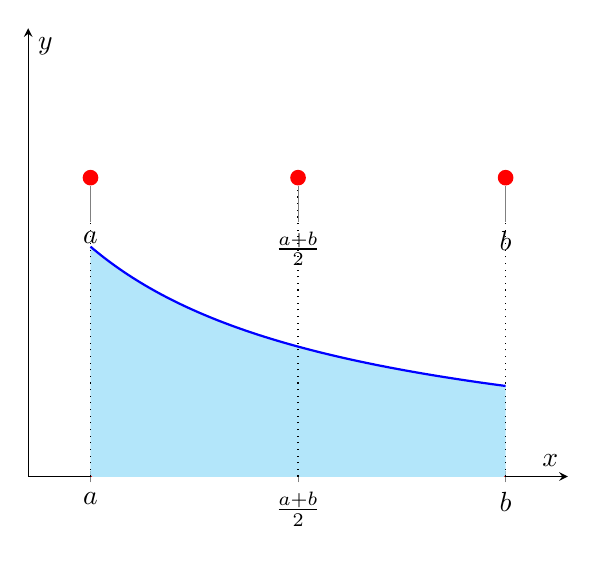
\begin{tikzpicture}
        \begin{axis}[
            axis lines=middle, 
            ytick=\empty, 
            ymax=1.5, ymin=0, xmax=2.6, xmin=0,
            xtick={0.3,1.3,2.3}, xticklabels={$a$,$\frac{a+b}{2}$,$b$},
            xlabel={$x$}, ylabel={$y$},
            every axis plot/.append style={thick}
        ]
    
        % Draw the function
        \addplot[name path=f, blue, domain=0.3:2.3, samples=100] {1/(x+1)};
    
        % Draw the Gauss-Legendre polynomial (quadratic)
        \addplot[name path=p2, red, domain=0.3:2.3] {0.5*(x-0.3)*(x-2.3)};
    
        % Fill between the function graph and the x-axis
        \addplot[cyan!30] fill between[of=f and p2];
    
        % Draw vertical lines for the interval
        \draw[dotted] (axis cs:0.3,0) -- (axis cs:0.3,1);
        \draw[dotted] (axis cs:2.3,0) -- (axis cs:2.3,1);
        \draw[dotted] (axis cs:1.3,0) -- (axis cs:1.3,1);
    
        % Place Gauss point markers
        \node[circle, fill=red, inner sep=2pt, pin=below:{$a$}] at (axis cs:0.3,1) {};
        \node[circle, fill=red, inner sep=2pt, pin=below:{$\frac{a+b}{2}$}] at (axis cs:1.3,1) {};
        \node[circle, fill=red, inner sep=2pt, pin=below:{$b$}] at (axis cs:2.3,1) {};
        
        \end{axis}
    \end{tikzpicture}
    \end{center}

    \subsection{Cuadratura Gaussiana}
    
    La \textbf{Cuadratura Gaussiana} es un método de integración numérica que utiliza nodos y pesos 
    específicos para aproximar la integral de una función en un intervalo $[a, b]$. La fórmula 
    general de la Cuadratura Gaussiana se expresa de la siguiente manera:
    
    \[
    \int_{a}^{b} f(x) \, dx \approx \sum_{i=1}^{n} w_i \cdot f(x_i)
    \]
    
    donde $w_i$ son los pesos asociados a los nodos $x_i$. La precisión de este método depende de 
    la elección de los nodos y pesos, que varían según el tipo de Cuadratura Gaussiana utilizada 
    (por ejemplo, Gauss-Legendre, Gauss-Hermite, Gauss-Laguerre, etc.). 
    \cite{smythnumerical}

    \section{Funciones de Prueba}
	\label{sec:funciones}
    Para evaluar y probar los métodos de integración numérica, consideramos las siguientes tres 	
    funciones de prueba:

    \begin{enumerate}
    
      \item \textbf{Función Polinómica:}
       Esta función polinómica simple se puede integrar analíticamente, lo que la hace útil para 
       comparaciones de precisión.
      \begin{equation}
      f(x) = x^2 + 3x - 5
      \end{equation}
    
      \item \textbf{Función racional:}
       Se optó por esta función por su simplicidad y la presencia de un término logarítmico en la 	
       integral, lo cual proporciona un buen ejemplo para evaluar la precisión de nuestras técnicas 
       numéricas. Además, la integración de funciones racionales es una práctica común en análisis 
       numérico y nos permite explorar cóo nuestros métodos se desempeñan en este contexto.
      \begin{equation}
      f(x) = \frac{1}{x + 1}
      \end{equation}

       \item \textbf{Función Trigonométrica:}
       La naturaleza trigonométrica de esta función nos permite probar cómo manejan los métodos
       numéricos el comportamiento oscilatorio.
      \begin{equation}
      f(x) = \sin(x)
      \end{equation}
    
    \end{enumerate}

    \subsection{Soluciones analíticas}
    Las soluciones exactas a las integrales de las funciones de prueba son las siguientes:

    \begin{enumerate}
     \item \textbf{Función polinómica:}
       Para calcular su integral definida, aplicamos la regla de potencias:
      
      \begin{equation}
      \int x^2 \, dx = \frac{1}{3}x^3 + C
      \end{equation}
      
      Donde \(C\) es una constante de integración.

      \item \textbf{Función racional:}
      
      La integral de la función racional se puede calcular analíticamente y su solución exacta es:
      
      \begin{equation}
      \int \frac{1}{x + 1} \,dx = \ln|x + 1| + C 
      \end{equation}
    
      \item \textbf{Función trigonométrica:}
      
      La integral de la función trigonométrica también es conocida y su solución exacta es:
      
      \begin{equation}
      \int \sin(x) \, dx = -\cos(x) + C
      \end{equation}
      
    \end{enumerate}

    \subsection{Reemplazo en intervalo}

    Tomando como punto de referencia un intervalo determinado para las tres funciones podemos
    comparar más fácil las soluciones analíticas con las funciones por métodos computacionales para 
    su posterior análisis.

    \begin{enumerate}
        \item \textbf{Función polinómica:}
        
        La integral definida en el intervalo \( [0, 2] \) es:
        \begin{equation}
        \int_{0}^{2} x^2 \, dx = \frac{1}{3}x^3 \Big|_{0}^{2} = \frac{1}{3}(2^3 - 0^3) = \frac{8}{3} = 2.666666667
        \end{equation}
    
        \item \textbf{Función racional:}
        
        La integral definida en el intervalo \( [0, 2] \) es:
        \begin{equation}
        \int_{0}^{2} \frac{1}{x + 1} \,dx = \ln|x + 1| \Big|_{0}^{2} = \ln(3) - \ln(1) = \ln(3) = 1.098612289
        \end{equation}
    
        \item \textbf{Función trigonométrica:}
        
        La integral definida en el intervalo \( [0, \pi] \) es:
        \begin{equation}
        \int_{0}^{\pi} \sin(x) \, dx = -\cos(x) \Big|_{0}^{\pi} = -\cos(\pi) + \cos(0) = 2
        \end{equation}
    \end{enumerate}

    
    \section{Implementación en Python}
	\label{sec:python}
    El desarrollo de implementaciones de cada técnica de integración numérica en el lenguaje de 
    programación Python pueden encontrarse en el  \underline{\href{https://github.com/nicolasgomeza7/tecnicasIntegracion}{repositorio}}.

    
    \section{Resultados}    
    \subsection{Eficiencia}
    
    En términos de eficiencia, medida como el tiempo de cálculo, se observaron los siguientes 
    resultados:
    
   \subsubsection{Función Trigonométrica}
    \begin{itemize}
        \item Método más rápido: Trapezoidal (6.3e-05 segundos).
        \item Orden de eficiencia: Trapezoidal $\geq$ Simpson $\geq$ Gaussiano.
    \end{itemize}
    
    \subsubsection{Función Polinomial}
    \begin{itemize}
        \item Método más rápido: Trapezoidal (2.1e-05 segundos).
        \item Orden de eficiencia: Trapezoidal $\geq$ Simpson $\geq$ Gaussiano.
    \end{itemize}
    
    \subsubsection{Función Racional}
    \begin{itemize}
        \item Método más rápido: Trapezoidal (1.5e-05 segundos).
        \item Orden de eficiencia: Trapezoidal $\geq$ Simpson $\geq$ Gaussiano.
    \end{itemize}

    
    \textbf{Observaciones:}
    En todas las funciones, el método Trapezoidal demostró ser el más eficiente en tiempo, seguido de cerca por el 
    método de Simpson, mientras que el método Gaussiano fue el menos eficiente.
    
    \subsection{Precisión}
    
    En cuanto a la precisión, medida como la cercanía a la solución analítica, se obtuvieron los siguientes hallazgos:
    
    \subsubsection{Función Polinomial}
    \begin{itemize}
        \item Aproximación más cercana: Gaussiano.
    \end{itemize}
    
    \subsubsection{Función Racional}
    \begin{itemize}
        \item Aproximación más cercana: Gaussiano.
    \end{itemize}
    
    \subsubsection{Función Trigonométrica}
    \begin{itemize}
        \item Aproximación más cercana: Gaussiano.
    \end{itemize}
    
    \textbf{Observaciones:}
    Para todas las funciones evaluadas, el método Gaussiano ofreció la aproximación más precisa a la solución analítica, a pesar de ser el más lento en términos de tiempo de cálculo.
    
    \subsection{Análisis de resultados}
    
    Se observa una clara compensación entre eficiencia y precisión en los métodos evaluados. Mientras que los métodos Trapezoidal y Simpson son más rápidos, el método Gaussiano proporciona resultados más precisos. La elección del método adecuado dependerá del equilibrio entre la necesidad de eficiencia (tiempo de cálculo) y precisión. Para funciones complejas o donde se requiere alta precisión, el tiempo adicional requerido por el método Gaussiano puede ser justificado, mientras que para respuestas rápidas con menor necesidad de precisión, los métodos Trapezoidal o Simpson pueden ser más adecuados.
    
     
    \section{Conclusiones}
    \label{sec:Conclusiones}
    Este proyecto ha explorado en profundidad la utilidad y aplicación de diversos métodos de integración numérica, subrayando su importancia en una amplia gama de campos científicos y de ingeniería. La integración numérica es fundamental en áreas donde las soluciones analíticas son difíciles o imposibles de obtener, como en la física computacional, la ingeniería, la economía, y en la modelización de fenómenos naturales y procesos industriales.

    A través del análisis de la Regla del Trapecio, la Regla de Simpson y la Cuadratura Gaussiana, hemos demostrado cómo cada técnica tiene sus propias ventajas y limitaciones, dependiendo del contexto de su aplicación. El método del Trapecio y la Regla de Simpson, debido a su mayor eficiencia en términos de tiempo de cálculo, son especialmente útiles en situaciones donde se requiere una respuesta rápida y la precisión absoluta no es crítica. Por otro lado, la Cuadratura Gaussiana, con su mayor precisión, es invaluable en investigaciones científicas y aplicaciones técnicas donde la exactitud es primordial.
    
    Este proyecto no solo ha proporcionado una comparación detallada de la eficiencia y precisión de estos métodos, sino que también ha brindado una plataforma para familiarizarse con su implementación en Python, un lenguaje de programación ampliamente utilizado en la ciencia de datos, la investigación y el desarrollo de software. La habilidad para implementar y comparar estos métodos es esencial para los ingenieros y científicos, permitiéndoles elegir la herramienta adecuada para sus necesidades específicas.
    
    En conclusión, los métodos de integración numérica son herramientas poderosas y flexibles en el análisis numérico. Su comprensión y correcta aplicación son cruciales para resolver problemas complejos en el mundo moderno, y este proyecto ha contribuido significativamente a este entendimiento, proporcionando insights valiosos y prácticos para su aplicación en diferentes escenarios.
    
    
    \printbibliography

\end{document}

